\documentclass{standalone}
\usepackage{tikz}
\usetikzlibrary{patterns, positioning}
\usepackage[sfdefault]{ClearSans} %% option 'sfdefault' activates Clear Sans as the default text font
\usepackage[T1]{fontenc}

\begin{document}
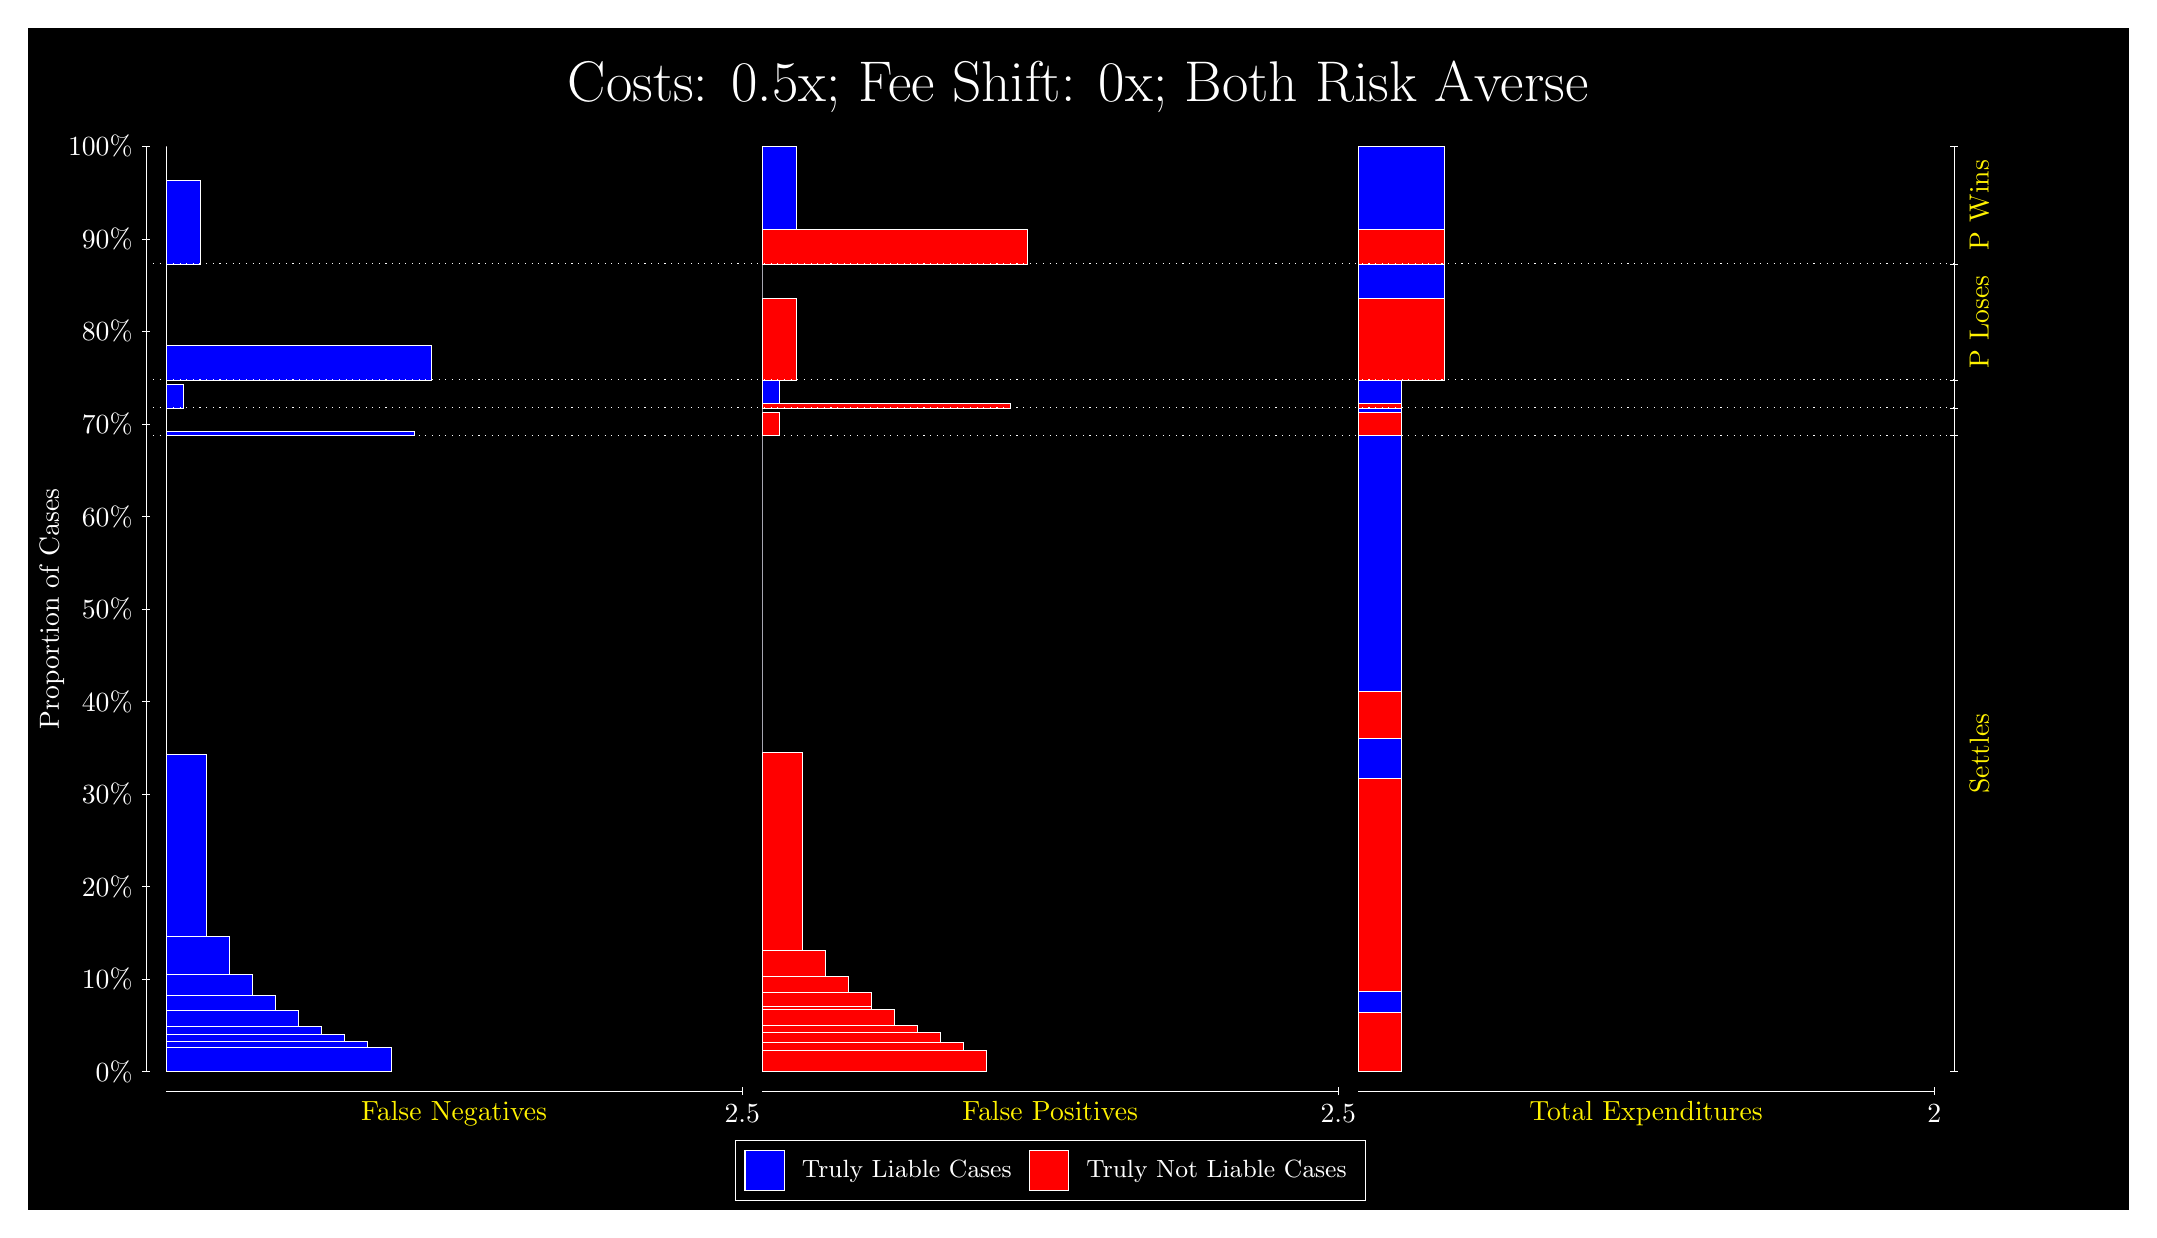
\begin{tikzpicture}
\draw[fill=black] (0,0) rectangle (26.667,15);
\draw[text=white] (0,13.5) rectangle (26.667,15) node[midway] {\huge Costs: 0.5x; Fee Shift: 0x; Both Risk Averse};
\draw[white, very thin] (1.5,1.75) -- (1.5,13.5);
\node[rotate=90, text=white, anchor=center] at (0.3, 7.625) {Proportion of Cases};
\draw[white, very thin] (1.45,1.75) -- (1.55,1.75);
\node[text=white, anchor=east] at (1.45, 1.75) {0\%};
\draw[white, very thin] (1.45,2.925) -- (1.55,2.925);
\node[text=white, anchor=east] at (1.45, 2.925) {10\%};
\draw[white, very thin] (1.45,4.1) -- (1.55,4.1);
\node[text=white, anchor=east] at (1.45, 4.1) {20\%};
\draw[white, very thin] (1.45,5.275) -- (1.55,5.275);
\node[text=white, anchor=east] at (1.45, 5.275) {30\%};
\draw[white, very thin] (1.45,6.45) -- (1.55,6.45);
\node[text=white, anchor=east] at (1.45, 6.45) {40\%};
\draw[white, very thin] (1.45,7.625) -- (1.55,7.625);
\node[text=white, anchor=east] at (1.45, 7.625) {50\%};
\draw[white, very thin] (1.45,8.8) -- (1.55,8.8);
\node[text=white, anchor=east] at (1.45, 8.8) {60\%};
\draw[white, very thin] (1.45,9.975) -- (1.55,9.975);
\node[text=white, anchor=east] at (1.45, 9.975) {70\%};
\draw[white, very thin] (1.45,11.15) -- (1.55,11.15);
\node[text=white, anchor=east] at (1.45, 11.15) {80\%};
\draw[white, very thin] (1.45,12.325) -- (1.55,12.325);
\node[text=white, anchor=east] at (1.45, 12.325) {90\%};
\draw[white, very thin] (1.45,13.5) -- (1.55,13.5);
\node[text=white, anchor=east] at (1.45, 13.5) {100\%};

\draw[white, very thin] (24.457,1.75) -- (24.457,13.5);
\draw[white, very thin] (24.407,1.75) -- (24.507,1.75);
\node[anchor=west] at (24.407, 1.75) {};
\draw[white, very thin] (24.407,9.8268) -- (24.507,9.8268);
\node[anchor=west] at (24.407, 9.8268) {};
\draw[white, very thin] (24.407,10.179) -- (24.507,10.179);
\node[anchor=west] at (24.407, 10.179) {};
\draw[white, very thin] (24.407,10.535) -- (24.507,10.535);
\node[anchor=west] at (24.407, 10.535) {};
\draw[white, very thin] (24.407,12.008) -- (24.507,12.008);
\node[anchor=west] at (24.407, 12.008) {};
\draw[white, very thin] (24.407,13.5) -- (24.507,13.5);
\node[anchor=west] at (24.407, 13.5) {};

\draw[white, very thin, fill=blue] (1.75,1.75) rectangle (4.6044,2.0582);
\draw[white, very thin, fill=blue] (1.75,2.0582) rectangle (4.3116,2.1351);
\draw[white, very thin, fill=blue] (1.75,2.1351) rectangle (4.0188,2.2275);
\draw[white, very thin, fill=blue] (1.75,2.2275) rectangle (3.7261,2.3247);
\draw[white, very thin, fill=blue] (1.75,2.3247) rectangle (3.4333,2.5269);
\draw[white, very thin, fill=blue] (1.75,2.5269) rectangle (3.1406,2.7133);
\draw[white, very thin, fill=blue] (1.75,2.7133) rectangle (2.8478,2.9812);
\draw[white, very thin, fill=blue] (1.75,2.9812) rectangle (2.5551,3.4721);
\draw[white, very thin, fill=blue] (1.75,3.4721) rectangle (2.2623,5.7769);
\draw[white, very thin, fill=red] (1.75,5.7769) rectangle (1.75,9.8268);
\draw[white, very thin, fill=blue] (1.75,9.8268) rectangle (4.8971,9.8857);
\draw[white, very thin, fill=red] (1.75,9.8857) rectangle (1.75,10.179);
\draw[white, very thin, fill=blue] (1.75,10.179) rectangle (1.9696,10.476);
\draw[white, very thin, fill=red] (1.75,10.476) rectangle (1.75,10.535);
\draw[white, very thin, fill=blue] (1.75,10.535) rectangle (5.1167,10.972);
\draw[white, very thin, fill=red] (1.75,10.972) rectangle (1.75,12.008);
\draw[white, very thin, fill=blue] (1.75,12.008) rectangle (2.1891,13.063);
\draw[white, very thin, fill=red] (1.75,13.063) rectangle (1.75,13.5);
\draw[white, very thin, fill=red] (9.3189,1.75) rectangle (12.173,2.0173);
\draw[white, very thin, fill=red] (9.3189,2.0173) rectangle (11.88,2.1263);
\draw[white, very thin, fill=red] (9.3189,2.1263) rectangle (11.588,2.2479);
\draw[white, very thin, fill=red] (9.3189,2.2479) rectangle (11.295,2.343);
\draw[white, very thin, fill=red] (9.3189,2.343) rectangle (11.002,2.5438);
\draw[white, very thin, fill=red] (9.3189,2.5438) rectangle (10.709,2.579);
\draw[white, very thin, fill=red] (9.3189,2.579) rectangle (10.709,2.751);
\draw[white, very thin, fill=red] (9.3189,2.751) rectangle (10.417,2.961);
\draw[white, very thin, fill=red] (9.3189,2.961) rectangle (10.124,3.296);
\draw[white, very thin, fill=red] (9.3189,3.296) rectangle (9.8312,5.7999);
\draw[white, very thin, fill=blue] (9.3189,5.7999) rectangle (9.3189,9.8268);
\draw[white, very thin, fill=red] (9.3189,9.8268) rectangle (9.5384,10.12);
\draw[white, very thin, fill=blue] (9.3189,10.12) rectangle (9.3189,10.179);
\draw[white, very thin, fill=red] (9.3189,10.179) rectangle (12.466,10.238);
\draw[white, very thin, fill=blue] (9.3189,10.238) rectangle (9.5384,10.535);
\draw[white, very thin, fill=red] (9.3189,10.535) rectangle (9.758,11.571);
\draw[white, very thin, fill=blue] (9.3189,11.571) rectangle (9.3189,12.008);
\draw[white, very thin, fill=red] (9.3189,12.008) rectangle (12.686,12.445);
\draw[white, very thin, fill=blue] (9.3189,12.445) rectangle (9.758,13.5);
\draw[white, very thin, fill=red] (16.888,1.75) rectangle (17.437,2.5022);
\draw[white, very thin, fill=blue] (16.888,2.5022) rectangle (17.437,2.7687);
\draw[white, very thin, fill=red] (16.888,2.7687) rectangle (17.437,5.4734);
\draw[white, very thin, fill=blue] (16.888,5.4734) rectangle (17.437,5.9837);
\draw[white, very thin, fill=red] (16.888,5.9837) rectangle (17.437,6.5768);
\draw[white, very thin, fill=blue] (16.888,6.5768) rectangle (17.437,9.8268);
\draw[white, very thin, fill=red] (16.888,9.8268) rectangle (17.437,10.12);
\draw[white, very thin, fill=blue] (16.888,10.12) rectangle (17.437,10.179);
\draw[white, very thin, fill=red] (16.888,10.179) rectangle (17.437,10.238);
\draw[white, very thin, fill=blue] (16.888,10.238) rectangle (17.437,10.535);
\draw[white, very thin, fill=red] (16.888,10.535) rectangle (17.986,11.571);
\draw[white, very thin, fill=blue] (16.888,11.571) rectangle (17.986,12.008);
\draw[white, very thin, fill=red] (16.888,12.008) rectangle (17.986,12.445);
\draw[white, very thin, fill=blue] (16.888,12.445) rectangle (17.986,13.5);
\draw[white, dotted] (1.5,9.8268) -- (24.457,9.8268);
\draw[white, dotted] (1.5,10.179) -- (24.457,10.179);
\draw[white, dotted] (1.5,10.535) -- (24.457,10.535);
\draw[white, dotted] (1.5,12.008) -- (24.457,12.008);
\draw[white, very thin] (1.75,1.5) -- (9.0689,1.5);
\node[text=yellow, anchor=north] at (5.4094, 1.5) {False Negatives};
\draw[white, very thin] (9.0689,1.45) -- (9.0689,1.55);
\node[text=white, anchor=north] at (9.0689, 1.45) {2.5};

\draw[white, very thin] (9.3189,1.5) -- (16.638,1.5);
\node[text=yellow, anchor=north] at (12.978, 1.5) {False Positives};
\draw[white, very thin] (16.638,1.45) -- (16.638,1.55);
\node[text=white, anchor=north] at (16.638, 1.45) {2.5};

\draw[white, very thin] (16.888,1.5) -- (24.207,1.5);
\node[text=yellow, anchor=north] at (20.547, 1.5) {Total Expenditures};
\draw[white, very thin] (24.207,1.45) -- (24.207,1.55);
\node[text=white, anchor=north] at (24.207, 1.45) {2};

\node[text=yellow, centered, rotate=90] at (24.777, 5.7884) {Settles};


\node[text=yellow, centered, rotate=90] at (24.777, 11.272) {P Loses};
\node[text=yellow, centered, rotate=90] at (24.777, 12.754) {P Wins};

\draw (12.978300999999998,1.5) node[draw=none] (baseCoordinate) {};
\begin{scope}[align=center]
        \matrix[scale=0.5, draw=white, below=0.5cm of baseCoordinate, nodes={draw}, column sep=0.1cm]{
            \node[rectangle, draw, minimum width=0.5cm, minimum height=0.5cm, fill=blue] {}; &
            \node[draw=none, font=\small, text=white] (B) {Truly Liable Cases}; &
            \node[rectangle, draw, minimum width=0.5cm, minimum height=0.5cm, fill=red] {}; &
            \node[draw=none, font=\small, text=white] (B) {Truly Not Liable Cases}; \\
            };
\end{scope}

\end{tikzpicture}
\end{document}